\section{加减法数字谜}

\title[第3讲\quad 加减法数字谜]{第3讲\quad 加减法数字谜} 
\author{}
\date{}
\begin{frame}
    \titlepage
\end{frame}

\begin{frame}
    \frametitle{课前测}
    \textit{用0、4、7这三个数字,能组成( )个没有重复数字的三位数.\\
    A.4\\ 
    B.5\\ 
    C.6}
\end{frame}

\begin{frame}
    \frametitle{课前测}
    \textit{用2、4、7、1 组成无重复数字的两位数,可能组成( )个.\\
    A.4\\ 
    B.8\\ 
    C.6}
\end{frame}

\begin{frame}
    \frametitle{课前测}
    \textit{用3、5、0、8 这4张数字卡片摆出的两位数,最小的奇数是多少?\\
    A.30\\ 
    B.33\\ 
    C.35}
\end{frame}

\begin{frame}
    \frametitle{知识梳理}
\end{frame}

\begin{frame}
    \frametitle{铺垫}
    \textit{相传在很久以前,由于没有很好的防虫措施,书上的算式常常被虫子吃掉一部分,所以人们在看书的时候,就得想办法,根据剩下的算式来判断被吃掉的数是几.后来人们就把这一类问题称为“虫蚀算”。\\
    在空格内填入适当的数字,使加法竖式成立}
    \begin{figure}[H] 
        \centering
        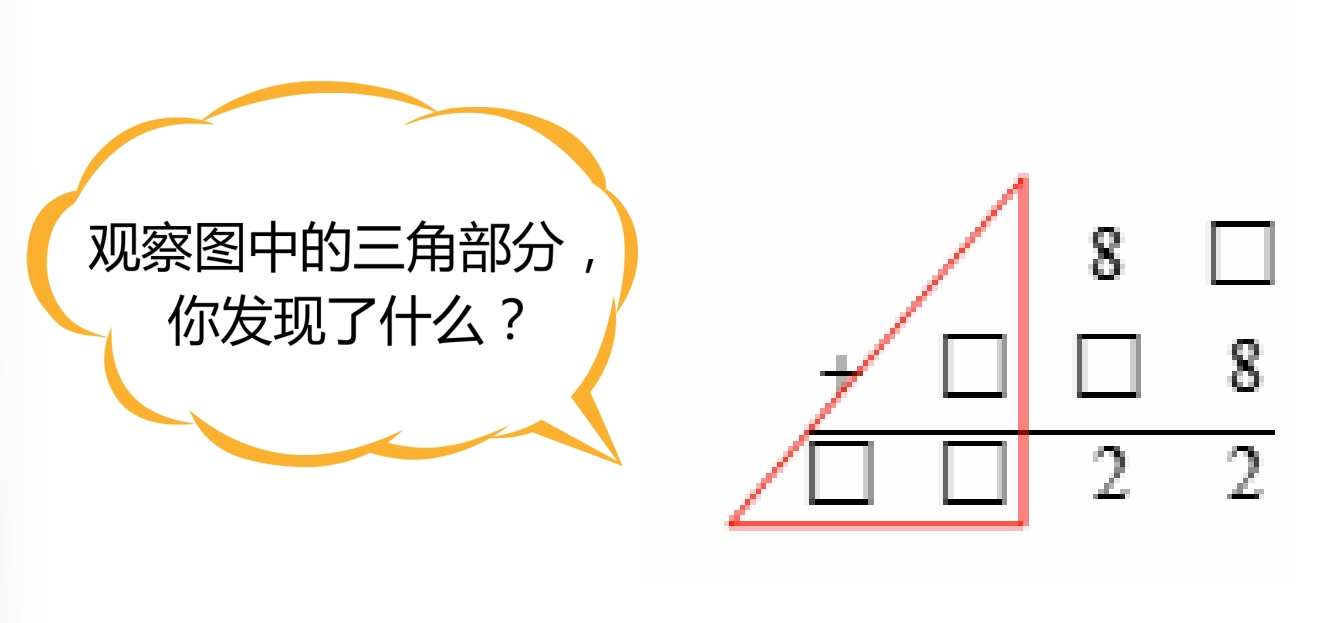
\includegraphics[width=0.5\textwidth]{./pics/Chapter_3/pudian.png}
    \end{figure}
\end{frame}

\begin{frame}
    \frametitle{探索1}
    \textit{(1)在空格内填入适当的数字,使图中的加法竖式成立.}
    \begin{figure}[H] 
        \centering
        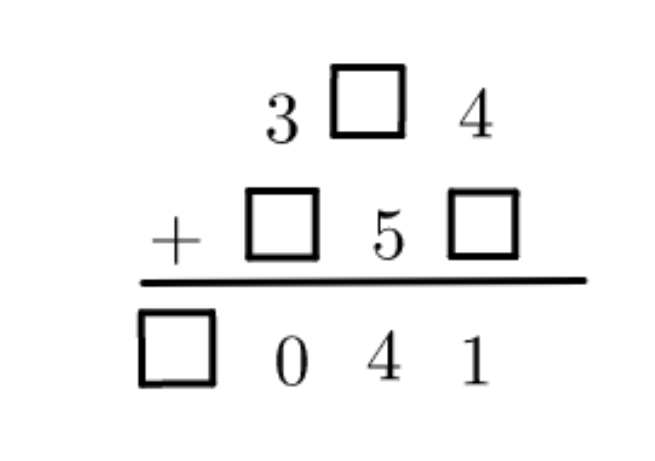
\includegraphics[width=0.5\textwidth]{./pics/Chapter_3/tansuo1_1.png}
    \end{figure}
\end{frame}

\begin{frame}
    \frametitle{探索1}
    \textit{(2)在空格内填入适当的数字,使图中的减法竖式成立.}
    \begin{figure}[H] 
        \centering
        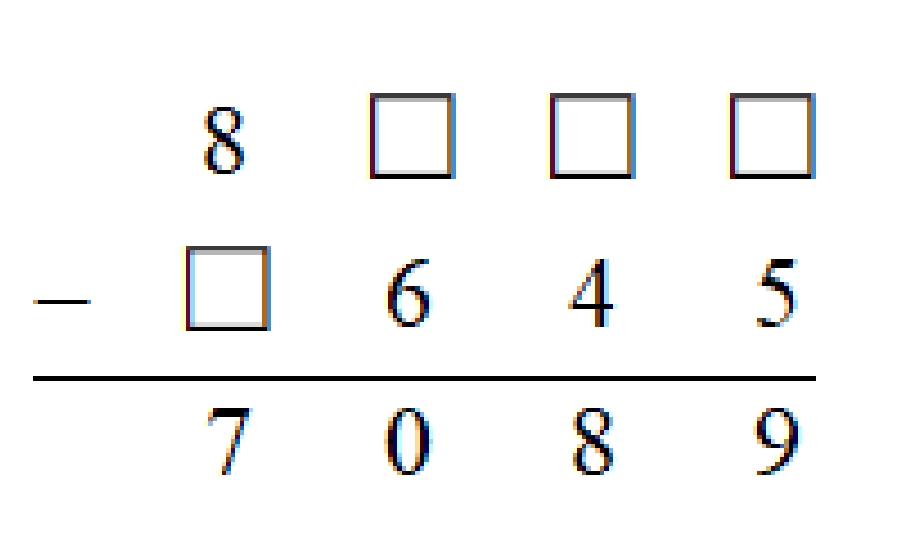
\includegraphics[width=0.5\textwidth]{./pics/Chapter_3/tansuo1_2.png}
    \end{figure}
\end{frame}

\begin{frame}
    \frametitle{捉虫时刻}
    \textit{请你给企鹅治病,并开出处方。}
    \begin{figure}[H] 
        \centering
        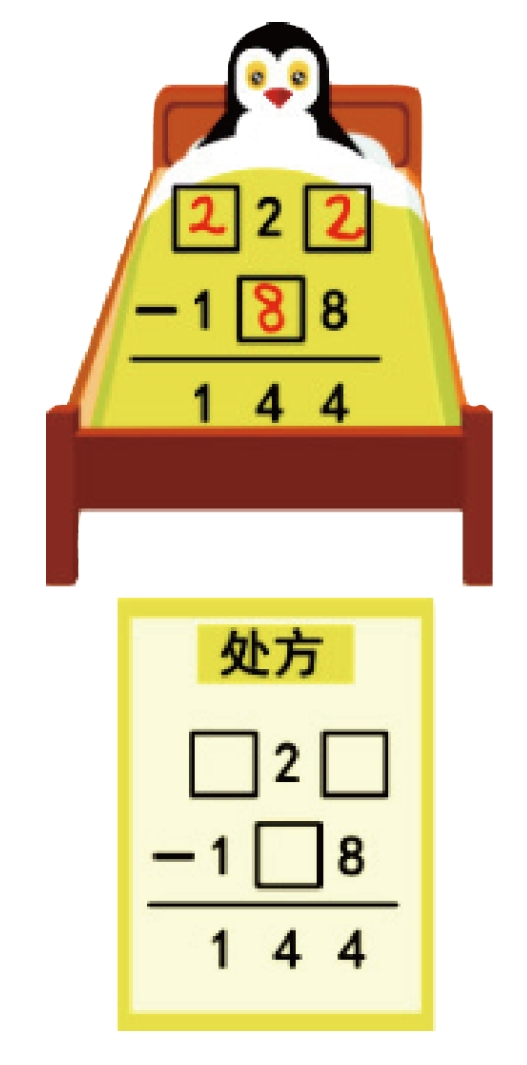
\includegraphics[width=0.2\textwidth]{./pics/Chapter_3/zhuochong.png}
    \end{figure}
\end{frame}

\begin{frame}
    \frametitle{探索2}
    \textit{(1)在空格内填入适当的数字,使图中的加法竖式成立。}
    
    \begin{figure}[H] 
        \centering
        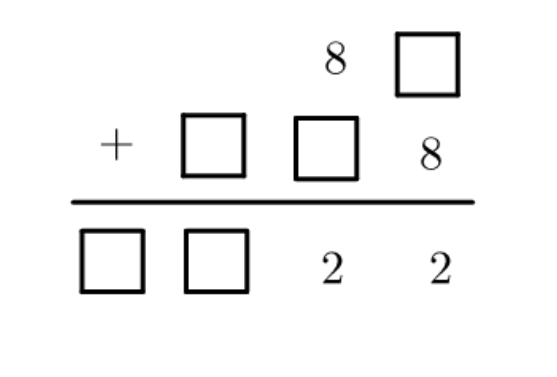
\includegraphics[width=0.5\textwidth]{./pics/Chapter_3/tansuo2_1.png}
    \end{figure}
\end{frame}

\begin{frame}
    \frametitle{探索2}
    \textit{(2)在空格内填入适当的数字,使图中的加法竖式成立}
    \begin{figure}[H] 
        \centering
        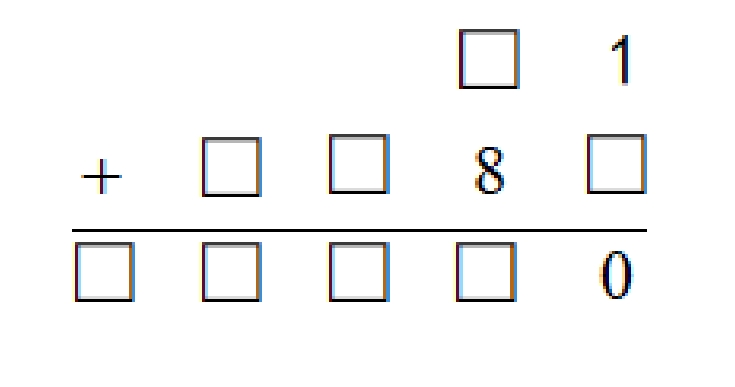
\includegraphics[width=0.5\textwidth]{./pics/Chapter_3/tansuo2_2.png}
    \end{figure}
\end{frame}

\begin{frame}
    \frametitle{探索3}
    \textit{(1)在空格内填入适当的数字,使图中的减法竖式成立。}
    \begin{figure}[H] 
        \centering
        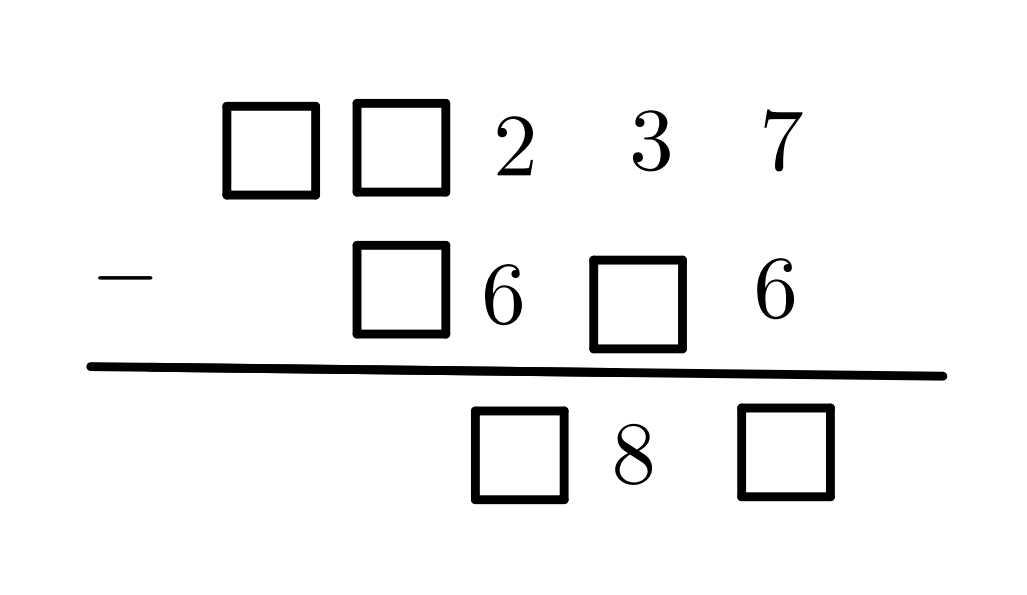
\includegraphics[width=0.5\textwidth]{./pics/Chapter_3/tansuo3_1.png}
    \end{figure}
\end{frame}

\begin{frame}
    \frametitle{探索3}
    \textit{(2)在空格内填入适当的数字,使图中的减法竖式成立。}
    \begin{figure}[H] 
        \centering
        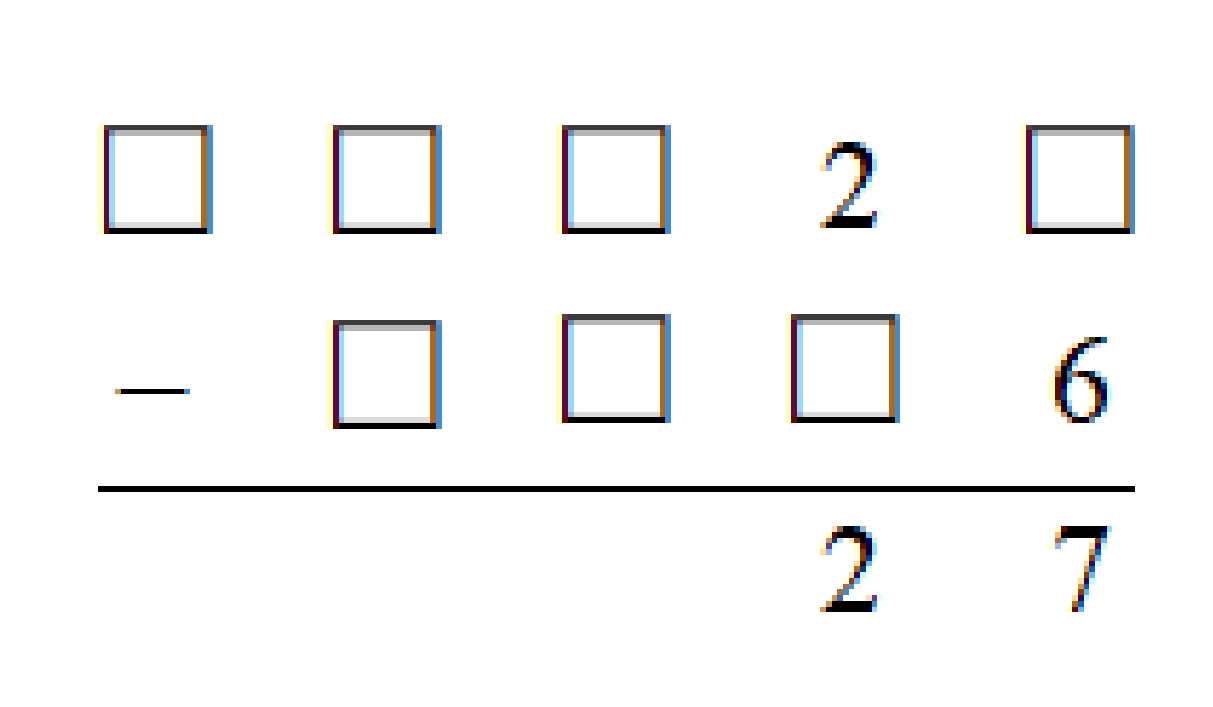
\includegraphics[width=0.5\textwidth]{./pics/Chapter_3/tansuo3_2.png}
    \end{figure}
\end{frame}

\begin{frame}
    \frametitle{课堂互动1}
    \textit{在下面算式的空格内,各填入一个合适的数字,使算式成立.最后结果是\underline{\hbox to 10mm{}}.}
    \begin{figure}[H] 
        \centering
        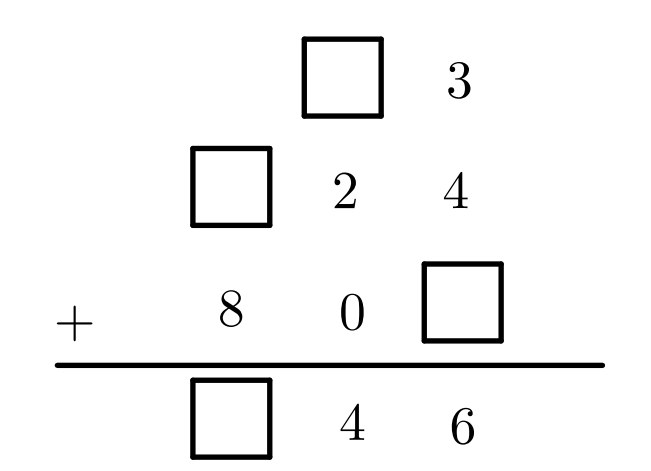
\includegraphics[width=0.5\textwidth]{./pics/Chapter_3/ketanghudong1.png}
    \end{figure}
\end{frame}

\begin{frame}
    \frametitle{课堂互动2}
    \textit{在下面算式的空格内,填入合适的数字,使算式成立.}
    \begin{figure}[H] 
        \centering
        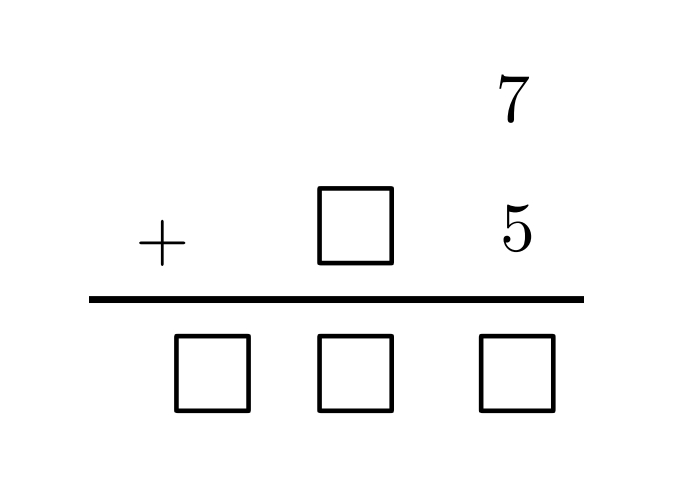
\includegraphics[width=0.5\textwidth]{./pics/Chapter_3/ketanghudong2.png}
    \end{figure}
\end{frame}

\begin{frame}
    \frametitle{课堂互动3}
    \textit{在下面算式的空格内,填入合适的数字,使算式成立.}
    \begin{figure}[H] 
        \centering
        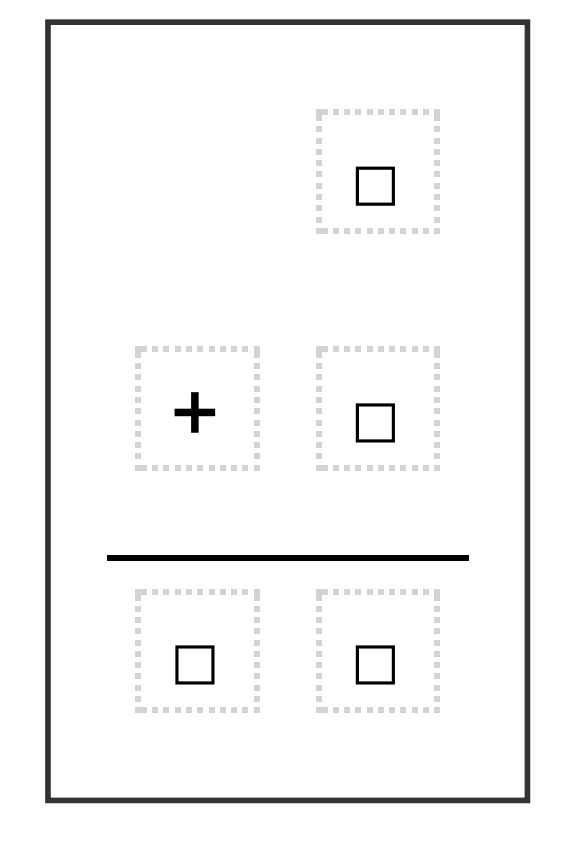
\includegraphics[width=0.3\textwidth]{./pics/Chapter_3/ketanghudong3.png}
    \end{figure}
\end{frame}


\begin{frame}
    \frametitle{MISSION 2}
    \vspace*{-2cm}
    \textit{在数字谜问题中,我们有什么样的分析方法呢?}
\end{frame}

\begin{frame}
    \frametitle{探索4}
    \textit{在下列的算式中,相同的符号代表相同的数字,不同的符号代表不同的数字,根据这个算式,可以推算出: $\square + \bigcirc + \triangle +$ \ding{73} $=$\underline{\hbox to 10mm{}}}
    \begin{figure}[H] 
        \centering
        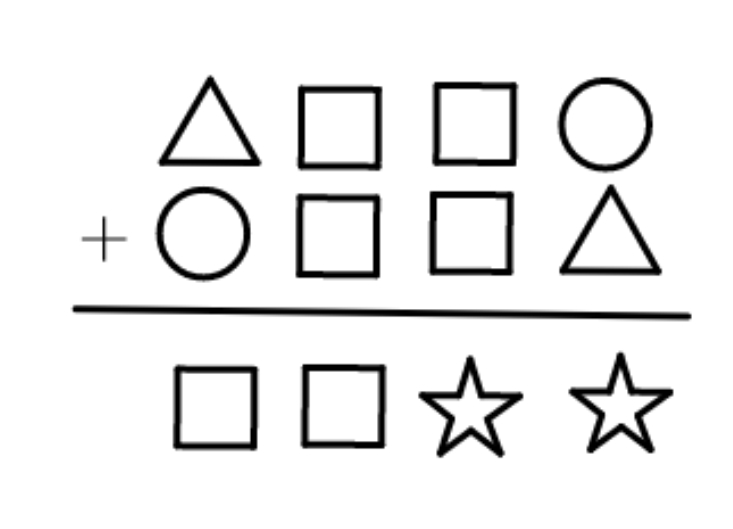
\includegraphics[width=0.4\textwidth]{./pics/Chapter_3/tansuo4.png}
    \end{figure}
\end{frame}

\begin{frame}
    \frametitle{探索5}
    \textit{在下面算式中,相同的字母代表相同的数字,不同的字母代表不同的数字,那么
    A=\underline{\hbox to 10mm{}}, 
    B=\underline{\hbox to 10mm{}},
    C=\underline{\hbox to 10mm{}},
    D=\underline{\hbox to 10mm{}}}
    \begin{figure}[H] 
        \centering
        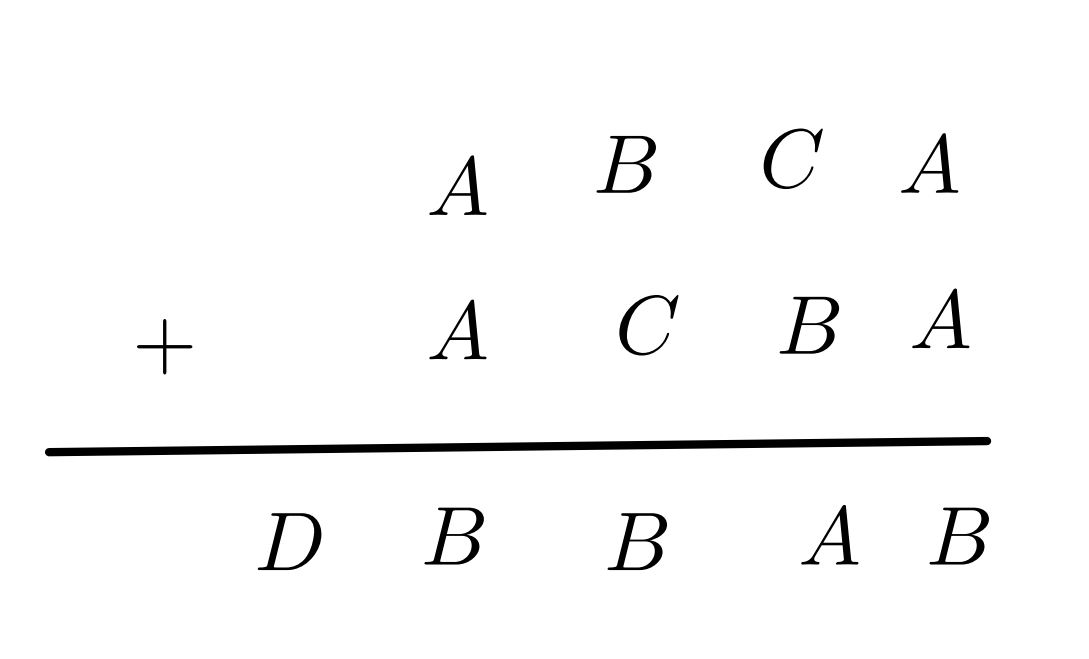
\includegraphics[width=0.5\textwidth]{./pics/Chapter_3/tansuo5.png}
    \end{figure}
\end{frame}

\begin{frame}
    \frametitle{探索6}
    \textit{下面的算式中, 不同的汉字表示不同的数字,相同的汉字表示相同的数字.如果``巧 + 解 + 数 + 字 + 谜 = 30'', 那么“巧解数字谜”所代表的五位数是多少?}
    \begin{figure}[H] 
        \centering
        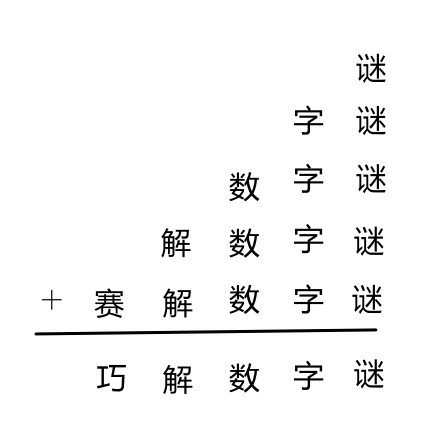
\includegraphics[width=0.4\textwidth]{./pics/Chapter_3/tansuo6.png}
    \end{figure}
    % 28965
\end{frame}

\begin{frame}
    \frametitle{探索7}
    \textit{在下面的竖式中,不同的汉字代表$0\sim 9$十个不同的数字,该竖式成立,则“听水无声”代表的四位数最小是\underline{\hbox to 10mm{}}.}
    \begin{figure}[H] 
        \centering
        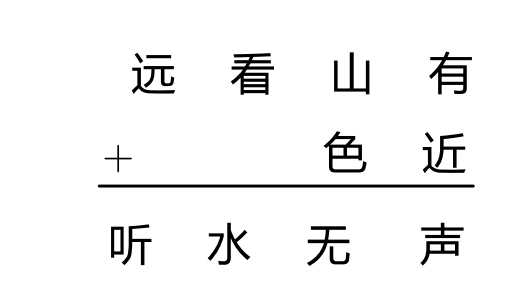
\includegraphics[width=0.5\textwidth]{./pics/Chapter_3/tansuo7.png}
    \end{figure}
    % 2034
\end{frame}

\begin{frame}
    \frametitle{探索8}
    \textit{如图,$A\sim J$分别代表 $0\sim 9$ 这10个数字,相同字母代表相同数字,不同字母代表不同数字,请问四位数GHIJ的最大值是多少?最小值是多少?}
    \begin{figure}[H] 
        \centering
        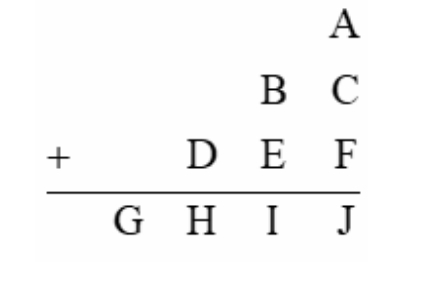
\includegraphics[width=0.5\textwidth]{./pics/Chapter_3/tansuo8.png}
    \end{figure}
    % 1062; 1026
\end{frame}

\begin{frame}
    \frametitle{补充2}
    \textit{在下面的算式中,A、B、C、D、E、F、G分别代表 $1\sim 9$ 中的数字,不同的字母代表不同的数字,恰使得加法算式成立.则三位数 $\overline{EFG}$ 的最大可能值是\underline{\hbox to 10mm{}}.}
    \begin{figure}[H] 
        \centering
        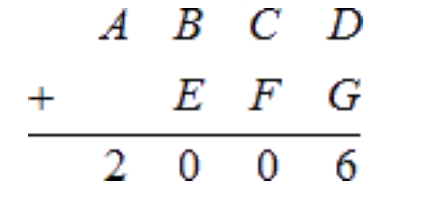
\includegraphics[width=0.5\textwidth]{./pics/Chapter_3/buchong2_1.png}
    \end{figure}
    % 659
\end{frame}

\begin{frame}
    \frametitle{补充2}
    \textit{$A+ \overline{AB} + \overline{ABC} + \overline{ABCD} = 4321$,且相同字母代表相同数字,不同字母代表不同数字,请问:A、B、C、D的和是多少?}
    \begin{figure}[H] 
        \centering
        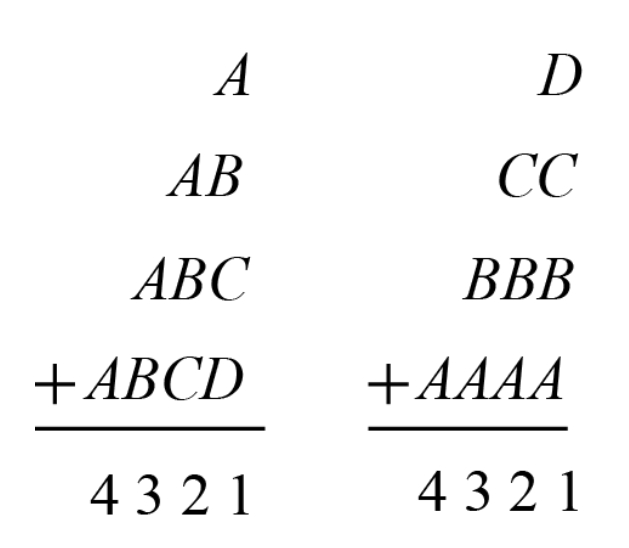
\includegraphics[width=0.5\textwidth]{./pics/Chapter_3/buchong2_2.png}
    \end{figure}
    % 21
\end{frame}

\begin{frame}
    \frametitle{补充2}
    \textit{公元 $\overline{ABCD}$ 年,美国数学会在洛杉矶举行微分几何大会,华人数学家丘成桐作为世界微分几何的新一代领导人出任大会主席.\\
    将一个四位数的数字顺序颠倒过来,得到一个新的四位数,新数比原数大 7902,在所有符合这样条件的四位数中, $\overline{ABCD}$ 是最大的,请问当时是公元多少年?}
    \begin{figure}[H] 
        \centering
        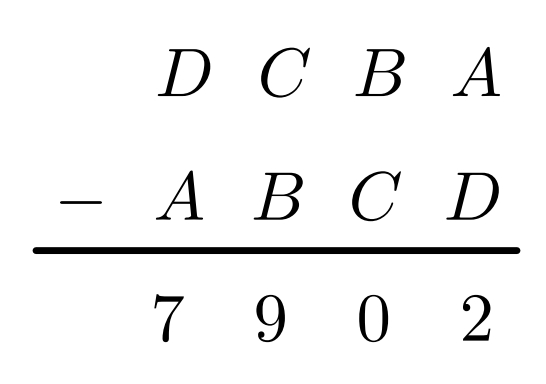
\includegraphics[width=0.5\textwidth]{./pics/Chapter_3/buchong2_3.png}
    \end{figure}
    % 1989
\end{frame}

\begin{frame}
    \frametitle{思维导图}
    \begin{figure}[H] 
        \centering
        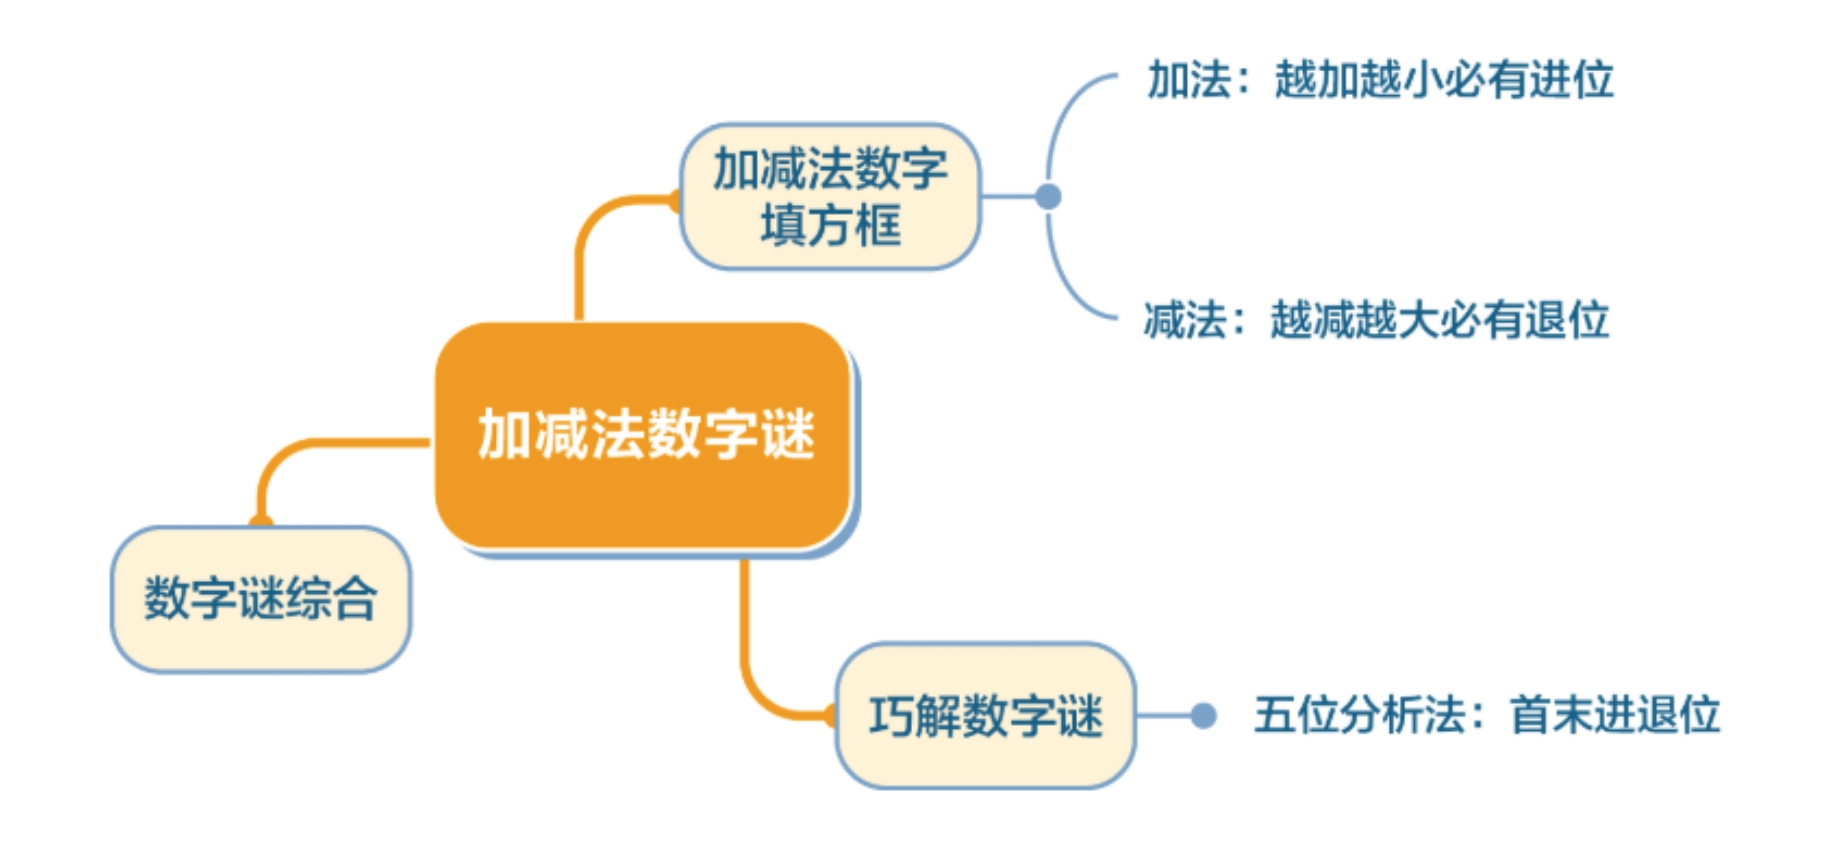
\includegraphics[width=1\textwidth]{./pics/Chapter_3/siweidaotu.png}
    \end{figure}
\end{frame}